\section{Experiments and Performance}
\label{experiments}

\subsection{Raytracing}

Initial tests of the raytracer.

\begin{figure}
\centering
\begin{subfigure}{.5\textwidth}
  \centering
  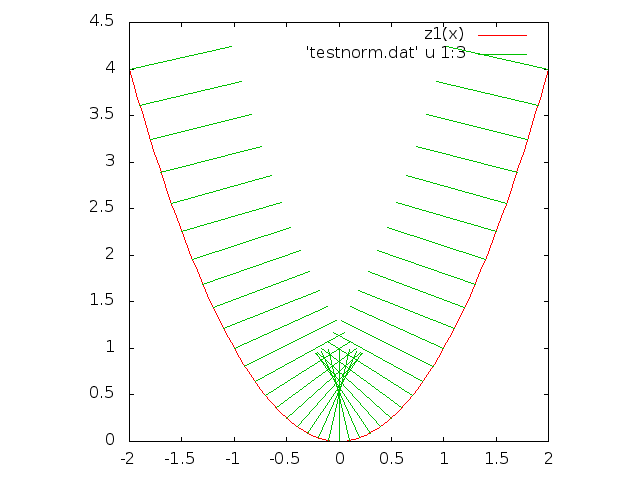
\includegraphics[width=7cm]{out.png}
  \caption{A norm}
  \label{fig:sub1}
\end{subfigure}%
\begin{subfigure}{.5\textwidth}
  \centering
  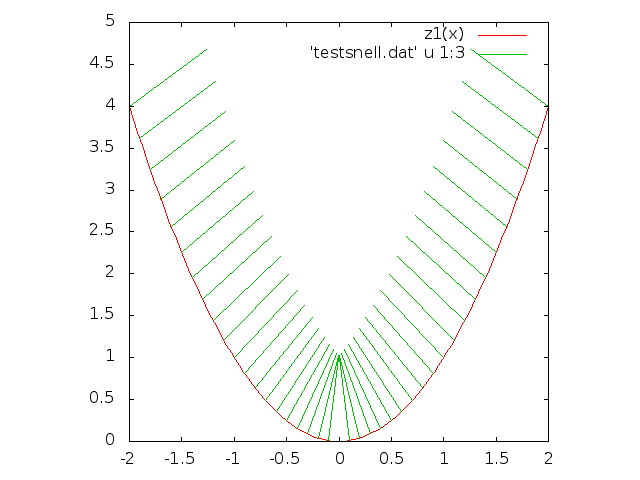
\includegraphics[width=7cm]{out2.png}
  \caption{A snell}
  \label{fig:sub2}
\end{subfigure}
\caption{A figure with two subfigures}
\label{fig:test}
\end{figure}

\begin{figure}
\centering
\begin{subfigure}{.5\textwidth}
  \centering
  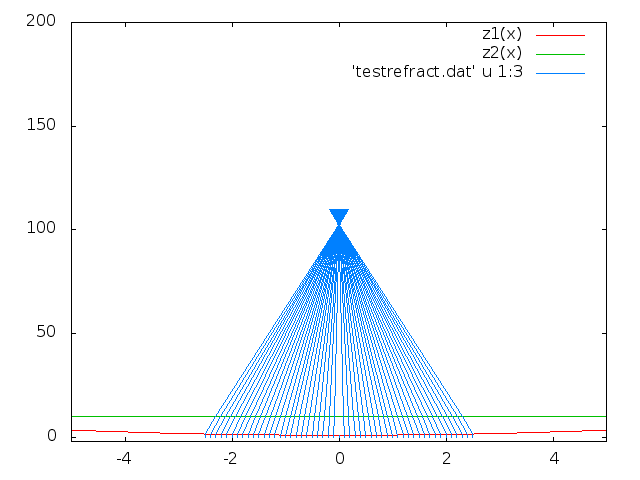
\includegraphics[width=7cm]{out4.png}
  \caption{A refract}
  \label{fig:sub3}
\end{subfigure}%
\begin{subfigure}{.5\textwidth}
  \centering
  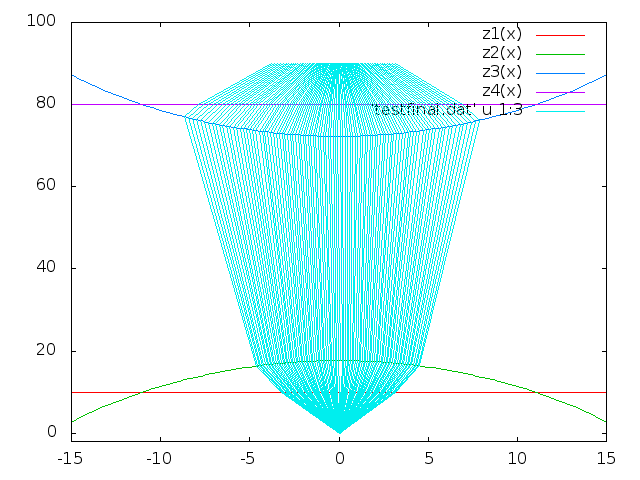
\includegraphics[width=7cm]{out5.png}
  \caption{A lenstest}
  \label{fig:sub4}
\end{subfigure}
\caption{A figure with two subfigures}
\label{fig:test2}
\end{figure}



\subsection{Training and Regression}

We had limited time to perform experiments due to the late arrival of our dataset.  However, the tests that we did perform clearly show that our distributed logistic classifier scales well to achieve significant performance gains.  In addition to provable performance gains, we also observed Gustafson's Law in action in that the available parallelism significantly increases with our problem size.

For our initial tests, we ran two training sets through the classifier.  The first training set was small (283M) and the second set was larger (~2.9G).  Our first goal was to observe the classification accuracy on of the classifier on the testing set.  Using the small training set, we were easily able to achieve 100\% accuracy.  This indicates that the amount of noise was insufficient and/or that there were not enough rays sampled to adequately obscure label partition boundaries.

Figures \ref{fig:small} \ref{fig:big} show performance gains for our initial tests.  We clearly see that while available parallelism levels out around 10 nodes with a student account on ACISS, the amount of available parallelism dramatically increases with our problem size.  The small dataset achieves a speedup of ~4 times relative to the serial execution while the larger dataset achieves ~9 times speed up.  This is an embarrassingly parallel problem with limited communication demands, so it is reassuring to see almost 10 times speedup with 10 times the computational power.  This implies that our implementation efficiently utilizes the parallel processing power to take advantage of available parallelism.

\begin{figure}[h]
\begin{center}
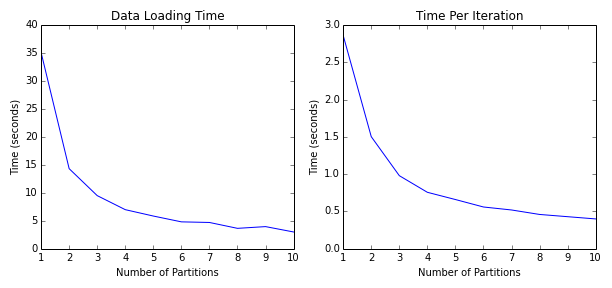
\includegraphics[scale=0.7]{small_metrics.png}
\caption{Performance gains for both data loading and iteration time on the small training set.}
\label{fig:small}
\end{center}
\end{figure}

\begin{figure}[h]
\begin{center}
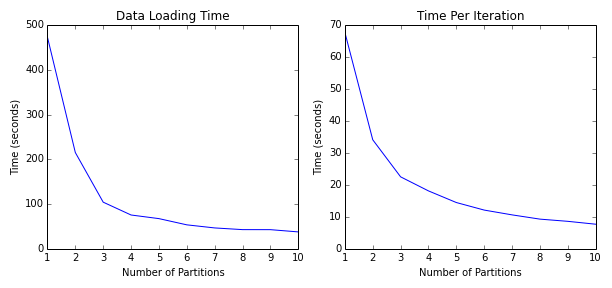
\includegraphics[scale=0.7]{big_metrics.png}
\caption{Performance gains for both data loading and iteration time on the large training set.}
\label{fig:big}
\end{center}
\end{figure}